%!TeX root = main.tex
\documentclass[main.tex]{subfiles}

\begin{document}

\chapter{Molecular simulation of adsorption}
\vspace*{-1\baselineskip}
\label{adsorption}

Adsorption is the physical phenomenon by which a molecule, the adsorbate, attaches to a surface, the adsorbent. One particular application of adsorption in the industry is for gas separation, by using an adsorbent that specifically binds one constituent of the target gas mixture more than the other.

In this chapter, we detail the nature of this phenomenon in the case of small gases in zeolites. We then explain the usual techniques which are used for its numerical simulation, as well as a possible alternative.

\section{Molecular description}

\subsection{Physisorption and chemisorption}

The atomic nature of adsorption depends on the kind of chemical interaction the supports it. On the one hand, if the adsorbate forms a strong (\textit{i.e.} covalent, sometimes ionic) bond with the adsorbent, then the adsorption is called a chemisorption, because it involves a chemical reaction. In that case, the surface is modified. On the other hand, if the adsorbate and adsorbent are only bond by a weak interaction, the adsorption is called a physisorption and the surface is left intact.

Chemisorption involves a stronger bond that physisorption, and is thus less reversible. Since it changes the surface of the adsorbent, it cannot be used industrially to separate large amounts of gas, as the adsorbent would need to be provided in equivalently large amount. It can however be used in the industry as an intermediate step of a catalytic cycle that ends up regenerating the surface. In our case however, we will implicitly refer to physisorption when mentioning adsorption.

\subsection{Adsorption sites in crystalline materials}

%At the atomic scale, the movement of species is driven by quantum mechanics. While the exact formulation of Schr\"odinger's equation cannot be solved exactly for more than a few particles, it has long been approximated to give a global understanding of the relevant phenomenons. In this context, the forces that play a key role in the non-bonded interactions of species are usually divided into two components: the charges of the species, which contribute a Coulomb term that evolves in $\frac1r$ with the distance between two particles, and a Van der Waals term that decays to zero much faster.

An adsorption site designates a particular space where the adsorbate is likely to remain trapped on the surface of the adsorbent. In other words, the interaction between the adsorbate and the adsorbent is maximally attractive when the adsorbate is located in one of the adsorption sites.

In the case of crystalline materials, adsorption sites can be identified through spectroscopy
%TODO expand and add examples

The position of the adsorption site depends on the adsorbent, but also the adsorbate. At very low density for example, a small polar molecule like \ce{H_2O} will preferentially adsorb in locations where it can orient itself to maximize the stabilizing Coulomb interaction of the framework. A large apolar molecule like a xylene on the other hand, will adsorb in locations that maximize its Van der Waals interactions with the adsorbent. Such sites are not necessarily related.

Moreover, the location of the adsorption sites becomes less relevant when the density of the adsorbate becomes high. Indeed, the adsorbate-adsorbate interactions can play a key role in the global adsorption capacity of a material, and the stronger these interactions, the more the internal structure of the adsorbate will reorganize to accommodate these interactions, which may displace some molecules from the ideal adsorption site.

Overall, the situation is quite different from the cationic sites, discussed in \cref{sitehopping}

\subsection{Small gases in zeolites}

Small gases such as \ce{CO_2}, \ce{N_2}, \ce{O_2}, \ce{CH_4} or \ce{Ar}, among others, are typical adsorbates that need to be separated for industrial purposes. In general, molecular sieves like zeolites can be used for this purpose

Given their rather similar sizes


\section{Grand Canonical Monte-Carlo}
\label{GCMC}

\subsection{Principle}

The adsorption capacity of a gas in a material at a fixed temperature and pressure is the number of molecules of gas that are retained by the material when in contact with a gas in these conditions, at equilibrium. Since it is a macroscopic observable $\mathcal O$, which can be experimentally measured, it can also be expressed as the statistical average of its microscopic counterpart $o$ in a well-chosen statistical ensemble. For the current case, the adsorption capacity results from a chemical equilibrium between the gas out of the material, at its given temperature $T$ and pressure $P$, and the gas in the pores of the material, at the same temperature $T$. The pressure of the gas in the material is an ill-defined concept, because it depends on the density of the gas, which itself is not uniform at any mesoscopic scale in a porous material. Instead, the chemical equilibrium translates to the equality of the chemical potentials $\mu$ of the gas in both conditions, hence $\mu$ is the relevant statistical variable to describe the system in the material, which accounts for the fixed gas pressure $P$ out of the material. Finally, we will focus on rigid crystalline materials, hence the volume $V$ of a unit cell can be used as an extensive variable to limit the size of the system.

The statistical ensemble resulting from the constraints of fixing the chemical potential $\mu$, the temperature $T$, and the volume $V$ is called the grand canonical ensemble. Similar to \cref{eq:canonicalensemble} used for the canonical ensemble (where the number of particles $N$ is fixed instead of their chemical potential $\mu$), $\mathcal O$ can be expressed using an integral over the microstates $(N,\boldsymbol p_N)$:
\[\mathcal O = \left<o\right> = \frac1\Xi\sum_N\int\!\text d{\boldsymbol p_N}\  o\left({\boldsymbol p_N}\right)\exp\left(-\beta \left(U\left({\boldsymbol p}\right) - \mu N\right)\right)\label{eq:grandcanonicalensemble}\]
where $N$ is the number of gas particles, $\boldsymbol p_N$ is their configuration, and $\Xi$ is the grand canonical partition function.

Likewise, this integral can be numerically evaluated by relying on a Monte-Carlo Markov Chain to provide a sequence of configurations $(N, \boldsymbol p_N)$ such that the statistical average $\left<o\right>$ can be retrieved by computing the arithmetic average of $o\left({\boldsymbol p_N}\right)$ over these configurations: this particular kind of simulation is naturally called a Grand Canonical Monte-Carlo (GCMC) simulation. In the specific case of the adsorption capacity, the microscopic function is simply $o\left({\boldsymbol p_N}\right) = N$, thus it is computed by running a GCMC simulation and simply averaging the number of particles in the system across the simulation.

\subsection{Implementation}

In practice, GCMC is implemented like a canonical MC simulation with one additional element: a swap MC move that can either insert or delete a particle. The insertion move simply consists in adding one additional gas particle to the system, while the deletion move removes one. If there are no particle in the systems anymore, the deletion move systematically fails; yet, it is crucial the probability of trying an insertion or a deletion remains equal independently of the number of particles in the system, to ensure micro-reversibility. For this reason, only the probability of trying a swap move is specified as a simulation parameter, while the probability of trying either an insertion or a deletion cannot be individually chosen and are necessarily equal to half the probability of a swap move.

The acceptance probability of a swap move is not decided purely on the basis of the difference of energy in the system, as is the case in \cref{eq:MCcanonicalaccept} for the canonical ensemble, because it also depends on the chemical potential $\mu$ of the system. With $N$, the number of particles in the system before the trial swap move, the acceptance probabilities for insertion and deletion are:
\[\begin{split}
	P_\text{accept}(\Delta E, N\to N+1) &= \min\paren{1,\ \frac{\beta\varphi P V}{N+1}\exp\paren{-\beta\Delta E}}\\
	P_\text{accept}(\Delta E, N\to N-1) &= \min\paren{1,\ \frac{N}{\beta\varphi P V}\exp\paren{-\beta\Delta E}}
\end{split}\]
The dependency to the chemical potential $\mu$ is conveyed by the pressure $P$ of the gas exterior to the zeolite. This value is corrected by the fugacity coefficient $\varphi$, which accounts for the difference between the real gas and the ideal gas model.

While the pressure $P$ and volume $V$ of the systems are simulation inputs, the fugacity coefficient $\varphi$ of the gas needs to be computed prior to the simulation. To do so, RASPA uses the Peng-Robinson equation of state, which is adequate for many common fluids. Since our range of gas applications is more restricted than the general-purpose RASPA software, we use the GERG-2008 [10.1021/je300655b] equation of state, which is the ISO standard for natural gases due to its accuracy compared to experimental measurements, with an extended validity range up to \qty{700}K and \qty{70}{MPa}, in the scope of our study.

\begin{figure}
	\centering
	\begin{subfigure}{0.5\columnwidth}
		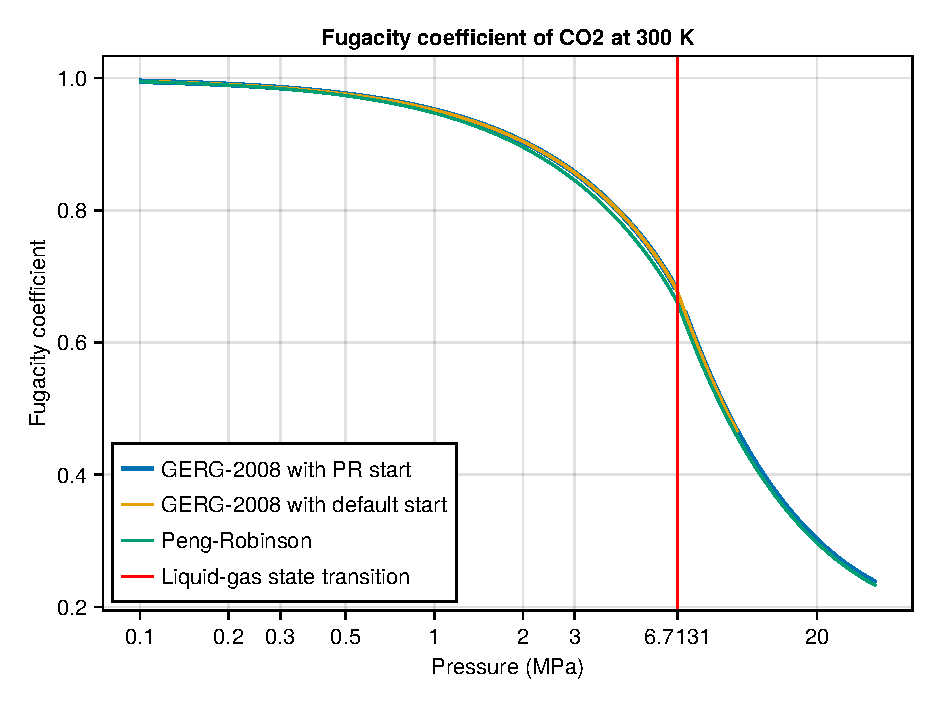
\includegraphics[width=\columnwidth]{figures/gcmc/fugacity.pdf}
		\subcaption{\ce{CO_2} at \qty{300}K}\label{fugacityCO2}
	\end{subfigure}\hfill%
	\begin{subfigure}{0.5\columnwidth}
		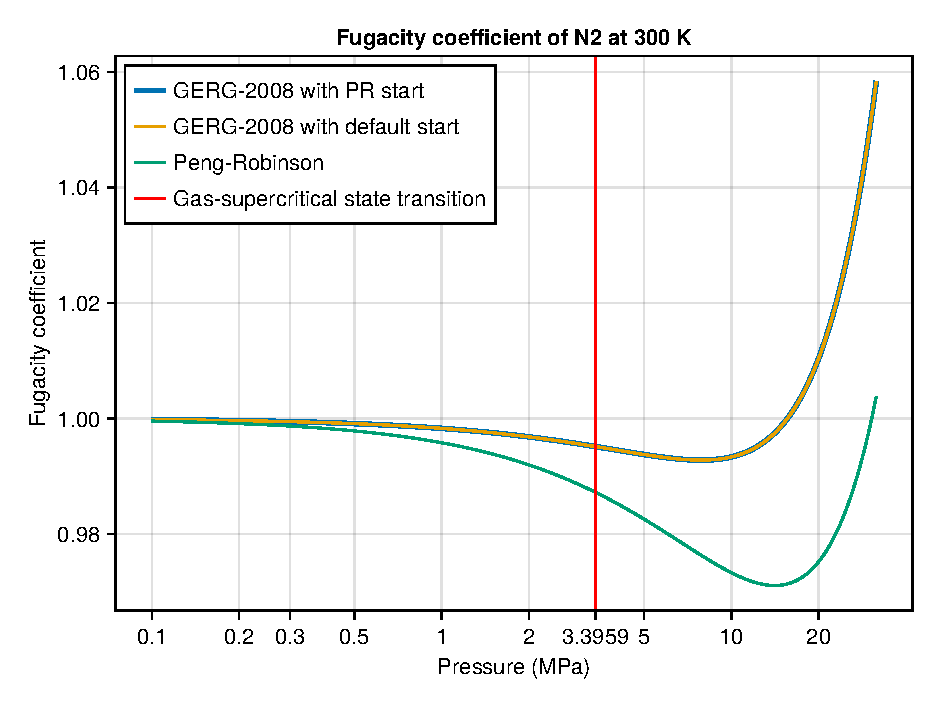
\includegraphics[width=\columnwidth]{figures/gcmc/fugacity_N2.pdf}
		\subcaption{\ce{N_2} at \qty{300}K}
	\end{subfigure}

	\begin{subfigure}{0.5\columnwidth}
		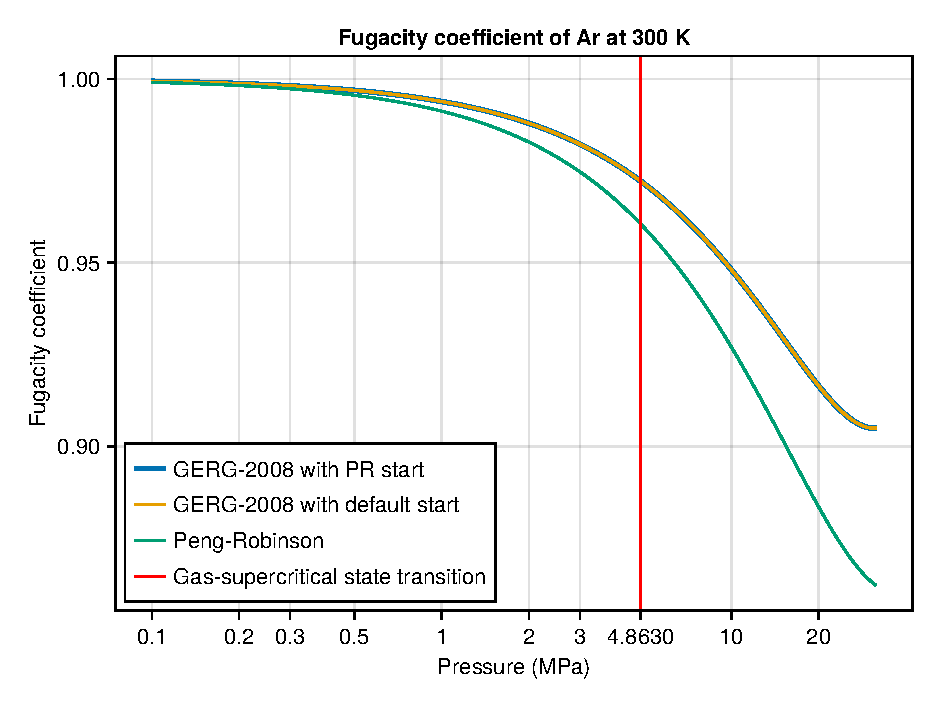
\includegraphics[width=\columnwidth]{figures/gcmc/fugacity_Ar.pdf}
		\subcaption{\ce{Ar} at \qty{300}K}
	\end{subfigure}\hfill%
	\begin{subfigure}{0.5\columnwidth}
		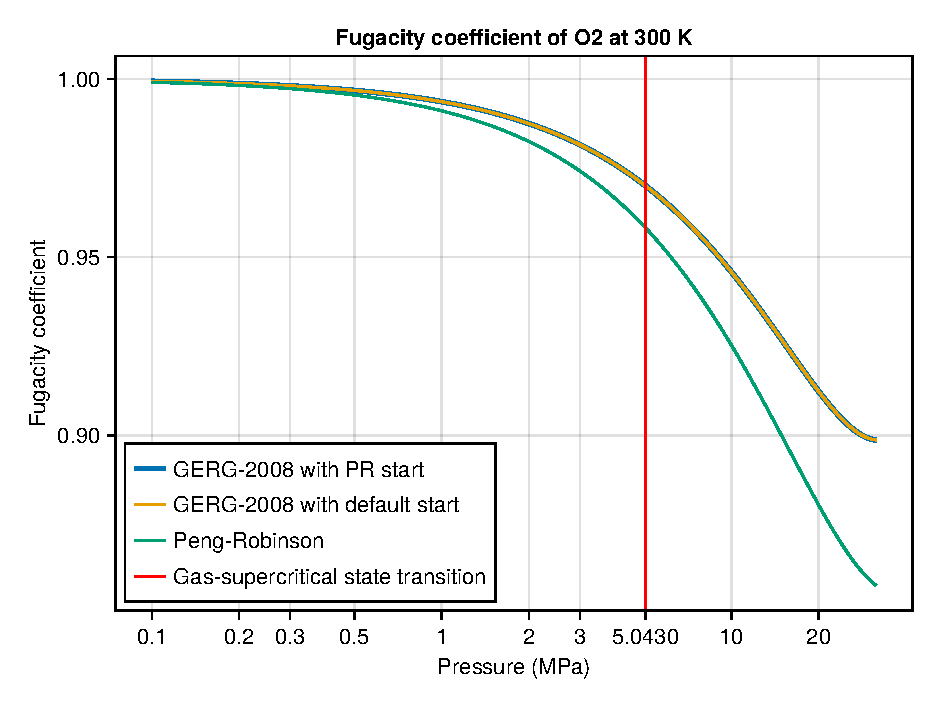
\includegraphics[width=\columnwidth]{figures/gcmc/fugacity_O2.pdf}
		\subcaption{\ce{O_2} at \qty{300}K}
	\end{subfigure}

	\caption{Fugacity coefficients of small gases computed with different \texttt{Clapeyron.jl} models}\label{fugacity}
\end{figure}

In terms of programming, the fugacity coefficient can directly be obtained from the \texttt{Clapeyron.jl} [10.1021/acs.iecr.2c00326] Julia package, which provides a convenient unified access to many useful thermodynamic tools. Due to the way it is implemented, Clapeyron.jl used to fail and return \texttt{NaN} instead of the valid fugacity coefficient for \ce{CO_2} at high pressures: to solve this issue, we do an initial volume computation for the gas in the target conditions using the Peng-Robinson model, and we use the result as the starting point to compute the coefficient with the GERG-2008 model. \Cref{fugacityCO2} illustrates the differences between these approaches: the latter allows to compute fugacities at any pressure except those very close to the critical point (\qty{304.13}K and \qty{7.3773}{MPa} for \ce{CO_2}), while the former simply fails at high pressures (above \qty1{MPa}). The other gases illustrated on \cref{fugacity} show that the Peng-Robinson fugacity is usually close but slightly lower than that obtained with GERG-2008, which would result in an equally slight underestimation of the adsorption capacity. The difference between the two equations of state remains in the uncertainty margin of the GCMC simulation however, so it should not lead to a visible difference in the measured adsorption capacity.

\subsection{Computational aspects}

Compared to canonical MC, the efficient implementation of GCMC poses the additional challenge of changing the number of particles across the simulation. This requires almost no accommodation for the computations that operate in the real space, \textit{i.e.} framework pre-computed grids, and pairwise interactions (including the direct part of Ewald summation). For these, the only adaptation consists in making the neighbour lists resizable, which is already implemented in \texttt{CellListMap.jl}, and otherwise keeping the list of atoms in the system up to date, to correctly check each pair of atoms. The direct part of Ewald summation falls in this category.

The reciprocal-space part of Ewald summation requires adapting the optimization described in \cref{energydifference} to account for the possible introduction or removal of a species. For such a move, both values of $S_{\boldsymbol k} = \sum_n q_ne^{i\boldsymbol k\cdot\boldsymbol r_n}$ before and after the swap need to be computed, exactly like in \cref{eq:reciprocal_move}. Likewise, the value before the swap is already stored in memory, but the computation of the new value is slightly different: instead of computing the difference as $\sum_n q_n\paren{e^{i\boldsymbol k\cdot\boldsymbol r'_n} - e^{i\boldsymbol k\cdot\boldsymbol r_n}}$, the difference is now $\pm\sum_{n\text{ swapped}} q_n e^{i\boldsymbol k\cdot\boldsymbol r_n}$. In the case of a deletion, each element of the latter is already stored in memory, whereas in the case of an insertion, this new computation is stored in a temporary place, like for any other trial move, ready to be stored permanently if the move is accepted.

The self-interaction term is no longer constant: each new molecule contributes a term equal to $\sum_m\frac{q_n q_m}{4\pi\varepsilon_0}\text{erf}\paren{\pnorm{\boldsymbol r_n - \boldsymbol r_m}}/\pnorm{\boldsymbol r_n - \boldsymbol r_m}$ where $m$ iterates over the atoms of the molecule. This term is computed once for each kind of molecules and stored, so that the contribution of the self-interaction term can be updated with a single addition or subtraction when a swap move occurs. Of course, any molecule whose number can vary must be electrically neutral to ensure the the overall system remains electrically neutral; this is also enforced in the code.

Another difference is the tail correction, which is not constant anymore either. %TODO

Overall, having a variable number of species requires extra bookkeeping, to make sure that all atoms are accounted for. To maximize performance in current computers, the data structures must have good cache locality: this means that, when memory needs to be read, it should be done in contiguous accesses as much as possible. For this purpose, the positions of the atoms, the $\kappa_{\boldsymbol k}$ factors, the precomputed $q_ne^{i\boldsymbol k\cdot \boldsymbol r_n}$ and $S_{\boldsymbol k}$, the self-interaction terms, etc., are all stored in tight arrays, with the appropriate indexing for each. When an atom is removed, there are two choices: either leave a gap in the array, and keep track separately of which parts of the array actually refer to a valid data if need be, or move the contents of the array to fill the gap.

Both algorithmic strategies have their merit, and warrant a trial to check which performs best. We did not take the time to implement both however, and instead chose the latter systematically, because it is slightly simpler to reason about. In practice, such an approach consists in replacing the content of the gap in the array by the data at the end of the array, before reducing the size of the array, and thus removing the temporarily duplicated data at the end. The indices relative to the content of the array also need to be updated. The complexity of each array update is thus proportional to the number of elements to remove, which is generally optimal. Insertions are operated at the end of the arrays, with an optimal complexity.

\section{GCMC on a grid}

\subsection{Principle}

\subsection{Validation}

\subsection{Limits and perspectives}

\end{document}
